\documentclass{standalone}
\usepackage{tikz}
\usetikzlibrary{patterns, positioning}

\begin{document}
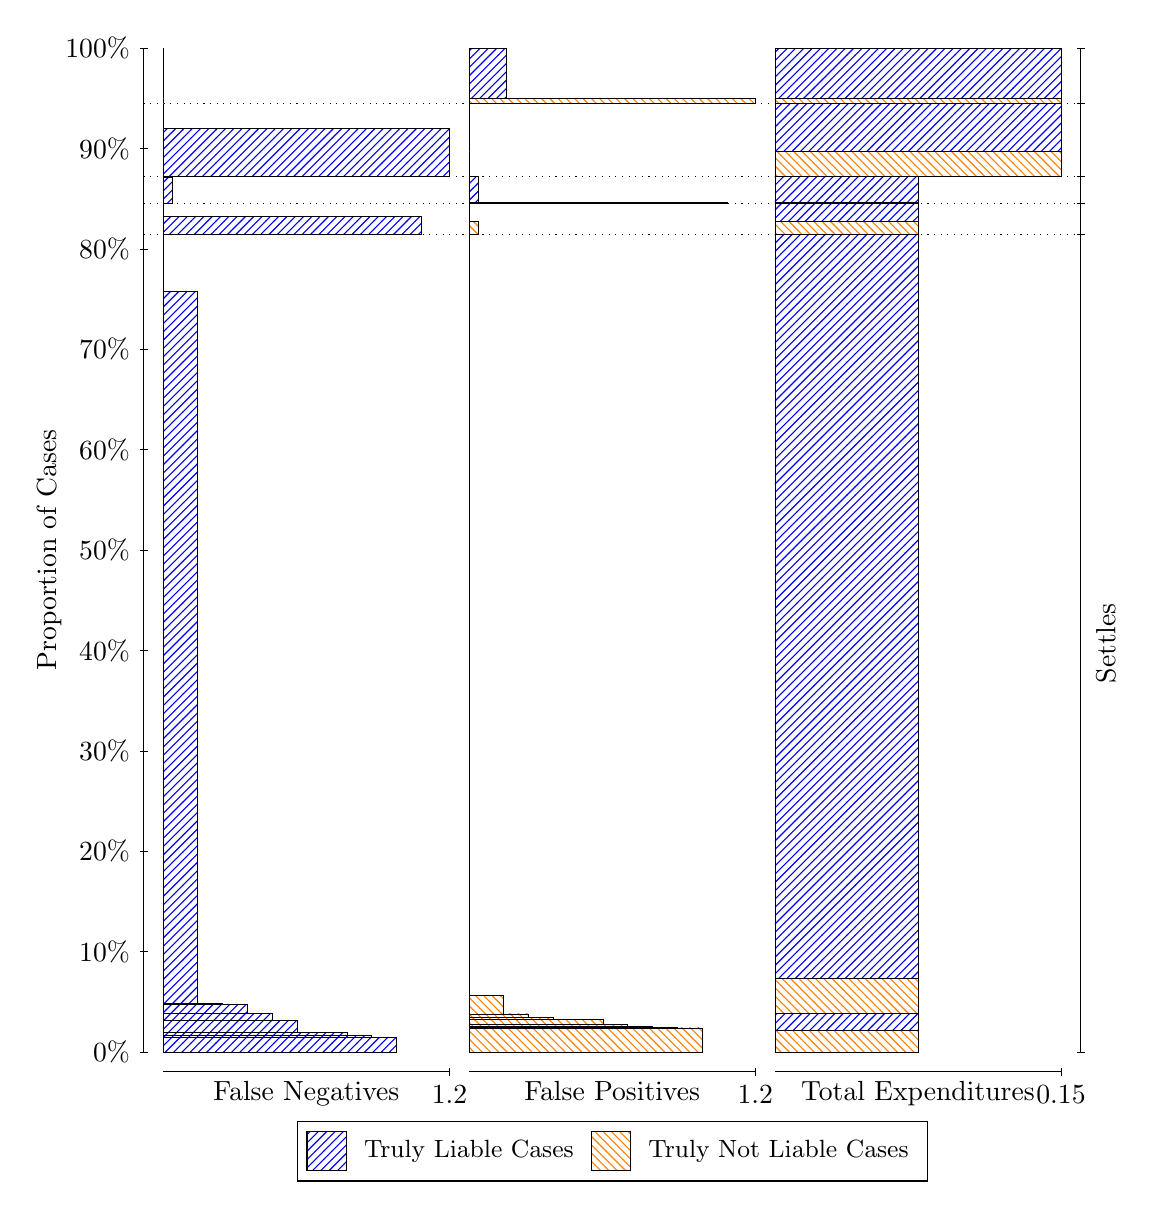
\begin{tikzpicture}
\draw[black, very thin] (1.5,1.75) -- (1.5,14.5);
\node[rotate=90, anchor=center] at (0.3, 8.125) {Proportion of Cases};
\draw[black, very thin] (1.45,1.75) -- (1.55,1.75);
\node[anchor=east] at (1.45, 1.75) {0\%};
\draw[black, very thin] (1.45,3.025) -- (1.55,3.025);
\node[anchor=east] at (1.45, 3.025) {10\%};
\draw[black, very thin] (1.45,4.3) -- (1.55,4.3);
\node[anchor=east] at (1.45, 4.3) {20\%};
\draw[black, very thin] (1.45,5.575) -- (1.55,5.575);
\node[anchor=east] at (1.45, 5.575) {30\%};
\draw[black, very thin] (1.45,6.85) -- (1.55,6.85);
\node[anchor=east] at (1.45, 6.85) {40\%};
\draw[black, very thin] (1.45,8.125) -- (1.55,8.125);
\node[anchor=east] at (1.45, 8.125) {50\%};
\draw[black, very thin] (1.45,9.4) -- (1.55,9.4);
\node[anchor=east] at (1.45, 9.4) {60\%};
\draw[black, very thin] (1.45,10.675) -- (1.55,10.675);
\node[anchor=east] at (1.45, 10.675) {70\%};
\draw[black, very thin] (1.45,11.95) -- (1.55,11.95);
\node[anchor=east] at (1.45, 11.95) {80\%};
\draw[black, very thin] (1.45,13.225) -- (1.55,13.225);
\node[anchor=east] at (1.45, 13.225) {90\%};
\draw[black, very thin] (1.45,14.5) -- (1.55,14.5);
\node[anchor=east] at (1.45, 14.5) {100\%};

\draw[black, very thin] (13.4,1.75) -- (13.4,14.5);
\draw[black, very thin] (13.35,1.75) -- (13.45,1.75);
\node[anchor=west] at (13.35, 1.75) {};
\draw[black, very thin] (13.35,12.131) -- (13.45,12.131);
\node[anchor=west] at (13.35, 12.131) {};
\draw[black, very thin] (13.35,12.531) -- (13.45,12.531);
\node[anchor=west] at (13.35, 12.531) {};
\draw[black, very thin] (13.35,12.872) -- (13.45,12.872);
\node[anchor=west] at (13.35, 12.872) {};
\draw[black, very thin] (13.35,13.796) -- (13.45,13.796);
\node[anchor=west] at (13.35, 13.796) {};
\draw[black, very thin] (13.35,14.5) -- (13.45,14.5);
\node[anchor=west] at (13.35, 14.5) {};

\draw[black, very thin, pattern color=blue, pattern=north east lines] (1.75,1.75) rectangle (4.712,1.9325);
\draw[black, very thin, pattern color=blue, pattern=north east lines] (1.75,1.9325) rectangle (4.396,1.9655);
\draw[black, very thin, pattern color=blue, pattern=north east lines] (1.75,1.9655) rectangle (4.0801,1.9952);
\draw[black, very thin, pattern color=blue, pattern=north east lines] (1.75,1.9952) rectangle (3.7641,2.0035);
\draw[black, very thin, pattern color=blue, pattern=north east lines] (1.75,2.0035) rectangle (3.4482,2.1558);
\draw[black, very thin, pattern color=blue, pattern=north east lines] (1.75,2.1558) rectangle (3.1322,2.2441);
\draw[black, very thin, pattern color=blue, pattern=north east lines] (1.75,2.2441) rectangle (2.8163,2.3588);
\draw[black, very thin, pattern color=blue, pattern=north east lines] (1.75,2.3588) rectangle (2.5004,2.3705);
\draw[black, very thin, pattern color=blue, pattern=north east lines] (1.75,2.3705) rectangle (2.1844,11.414);
\draw[black, very thin, pattern color=orange, pattern=north west lines] (1.75,11.414) rectangle (1.75,12.131);
\draw[black, very thin, pattern color=blue, pattern=north east lines] (1.75,12.131) rectangle (5.0279,12.363);
\draw[black, very thin, pattern color=orange, pattern=north west lines] (1.75,12.363) rectangle (1.75,12.531);
\draw[black, very thin, pattern color=blue, pattern=north east lines] (1.75,12.531) rectangle (1.8685,12.863);
\draw[black, very thin, pattern color=orange, pattern=north west lines] (1.75,12.863) rectangle (1.75,12.872);
\draw[black, very thin, pattern color=blue, pattern=north east lines] (1.75,12.872) rectangle (5.3833,13.481);
\draw[black, very thin, pattern color=orange, pattern=north west lines] (1.75,13.481) rectangle (1.75,13.796);
\draw[black, very thin, pattern color=orange, pattern=north west lines] (1.75,13.796) rectangle (1.75,13.862);
\draw[black, very thin, pattern color=blue, pattern=north east lines] (1.75,13.862) rectangle (1.75,14.5);
\draw[black, very thin, pattern color=orange, pattern=north west lines] (5.6333,1.75) rectangle (8.5953,2.0558);
\draw[black, very thin, pattern color=orange, pattern=north west lines] (5.6333,2.0558) rectangle (8.2793,2.0583);
\draw[black, very thin, pattern color=orange, pattern=north west lines] (5.6333,2.0583) rectangle (7.9634,2.0776);
\draw[black, very thin, pattern color=orange, pattern=north west lines] (5.6333,2.0776) rectangle (7.6475,2.0985);
\draw[black, very thin, pattern color=orange, pattern=north west lines] (5.6333,2.0985) rectangle (7.3315,2.1591);
\draw[black, very thin, pattern color=orange, pattern=north west lines] (5.6333,2.1591) rectangle (7.0156,2.1641);
\draw[black, very thin, pattern color=orange, pattern=north west lines] (5.6333,2.1641) rectangle (7.0156,2.1644);
\draw[black, very thin, pattern color=orange, pattern=north west lines] (5.6333,2.1644) rectangle (6.6996,2.1929);
\draw[black, very thin, pattern color=orange, pattern=north west lines] (5.6333,2.1929) rectangle (6.3837,2.2342);
\draw[black, very thin, pattern color=orange, pattern=north west lines] (5.6333,2.2342) rectangle (6.0678,2.4669);
\draw[black, very thin, pattern color=blue, pattern=north east lines] (5.6333,2.4669) rectangle (5.6333,12.131);
\draw[black, very thin, pattern color=orange, pattern=north west lines] (5.6333,12.131) rectangle (5.7518,12.298);
\draw[black, very thin, pattern color=blue, pattern=north east lines] (5.6333,12.298) rectangle (5.6333,12.531);
\draw[black, very thin, pattern color=orange, pattern=north west lines] (5.6333,12.531) rectangle (8.9112,12.54);
\draw[black, very thin, pattern color=blue, pattern=north east lines] (5.6333,12.54) rectangle (5.7518,12.872);
\draw[black, very thin, pattern color=orange, pattern=north west lines] (5.6333,12.872) rectangle (5.6333,13.187);
\draw[black, very thin, pattern color=blue, pattern=north east lines] (5.6333,13.187) rectangle (5.6333,13.796);
\draw[black, very thin, pattern color=orange, pattern=north west lines] (5.6333,13.796) rectangle (9.2667,13.862);
\draw[black, very thin, pattern color=blue, pattern=north east lines] (5.6333,13.862) rectangle (6.1072,14.5);
\draw[black, very thin, pattern color=orange, pattern=north west lines] (9.5167,1.75) rectangle (11.333,2.0239);
\draw[black, very thin, pattern color=blue, pattern=north east lines] (9.5167,2.0239) rectangle (11.333,2.2394);
\draw[black, very thin, pattern color=orange, pattern=north west lines] (9.5167,2.2394) rectangle (11.333,2.6823);
\draw[black, very thin, pattern color=blue, pattern=north east lines] (9.5167,2.6823) rectangle (11.333,12.131);
\draw[black, very thin, pattern color=orange, pattern=north west lines] (9.5167,12.131) rectangle (11.333,12.298);
\draw[black, very thin, pattern color=blue, pattern=north east lines] (9.5167,12.298) rectangle (11.333,12.531);
\draw[black, very thin, pattern color=orange, pattern=north west lines] (9.5167,12.531) rectangle (11.333,12.54);
\draw[black, very thin, pattern color=blue, pattern=north east lines] (9.5167,12.54) rectangle (11.333,12.872);
\draw[black, very thin, pattern color=orange, pattern=north west lines] (9.5167,12.872) rectangle (13.15,13.187);
\draw[black, very thin, pattern color=blue, pattern=north east lines] (9.5167,13.187) rectangle (13.15,13.796);
\draw[black, very thin, pattern color=orange, pattern=north west lines] (9.5167,13.796) rectangle (13.15,13.862);
\draw[black, very thin, pattern color=blue, pattern=north east lines] (9.5167,13.862) rectangle (13.15,14.5);
\draw[black, dotted] (1.5,12.131) -- (13.4,12.131);
\draw[black, dotted] (1.5,12.531) -- (13.4,12.531);
\draw[black, dotted] (1.5,12.872) -- (13.4,12.872);
\draw[black, dotted] (1.5,13.796) -- (13.4,13.796);
\draw[black, very thin] (1.75,1.5) -- (5.3833,1.5);
\node[anchor=north] at (3.5667, 1.5) {False Negatives};
\draw[black, very thin] (5.3833,1.45) -- (5.3833,1.55);
\node[anchor=north] at (5.3833, 1.45) {1.2};

\draw[black, very thin] (5.6333,1.5) -- (9.2667,1.5);
\node[anchor=north] at (7.45, 1.5) {False Positives};
\draw[black, very thin] (9.2667,1.45) -- (9.2667,1.55);
\node[anchor=north] at (9.2667, 1.45) {1.2};

\draw[black, very thin] (9.5167,1.5) -- (13.15,1.5);
\node[anchor=north] at (11.333, 1.5) {Total Expenditures};
\draw[black, very thin] (13.15,1.45) -- (13.15,1.55);
\node[anchor=north] at (13.15, 1.45) {0.15};

\node[black, centered, rotate=90] at (13.72, 6.9404) {Settles};





\draw (7.449999999999999,1.5) node[draw=none] (baseCoordinate) {};
\begin{scope}[align=center]
        \matrix[scale=0.5, draw=black, below=0.5cm of baseCoordinate, nodes={draw}, column sep=0.1cm]{
            \node[rectangle, draw, minimum width=0.5cm, minimum height=0.5cm, pattern=north east lines, pattern color=blue] {}; &
            \node[draw=none, font=\small] (B) {Truly Liable Cases}; &
            \node[rectangle, draw, minimum width=0.5cm, minimum height=0.5cm, pattern=north west lines, pattern color=orange] {}; &
            \node[draw=none, font=\small] (B) {Truly Not Liable Cases}; \\
            };
\end{scope}

\end{tikzpicture}
\end{document}